\chapter{利用例}
\label{chap:riyourei}

本章ではDrawWikiの利用例を紹介する。

\newpage

手書きメモ・イラストの内部に別の画像へのリンクが埋め込めるというDrawWikiの機能を活かし、次のように利用した。


\section{グラフィカルなアイデアスケッチやメモ}


\section{スケッチによるソフトウェアのモックアップの作成}
\label{drawiki:mockup}
ソフトウェアの画面や挙動を設計する際に、柔軟な表現が可能な手書きスケッチを用いることが有効な
デザインプラクティスとして知られている。
DrawWikiを開発する際も、機能や画面全体のデザインを考える際にDrawWikiを用いてスケッチを行いながら検討した。
リンクが埋め込まれた要素をクリックするとリンク先の画像が表示されることから、これをインタラクションや画面遷移に見立てることにより
図\ref{fig:protodrawwiki}のようなナビゲーションを伴ったソフトウェアのモックアップを手書きスケッチによって作成することができる。

\begin{figure}[H] \begin{minipage}{0.5\hsize}
                      \begin{center} \fbox {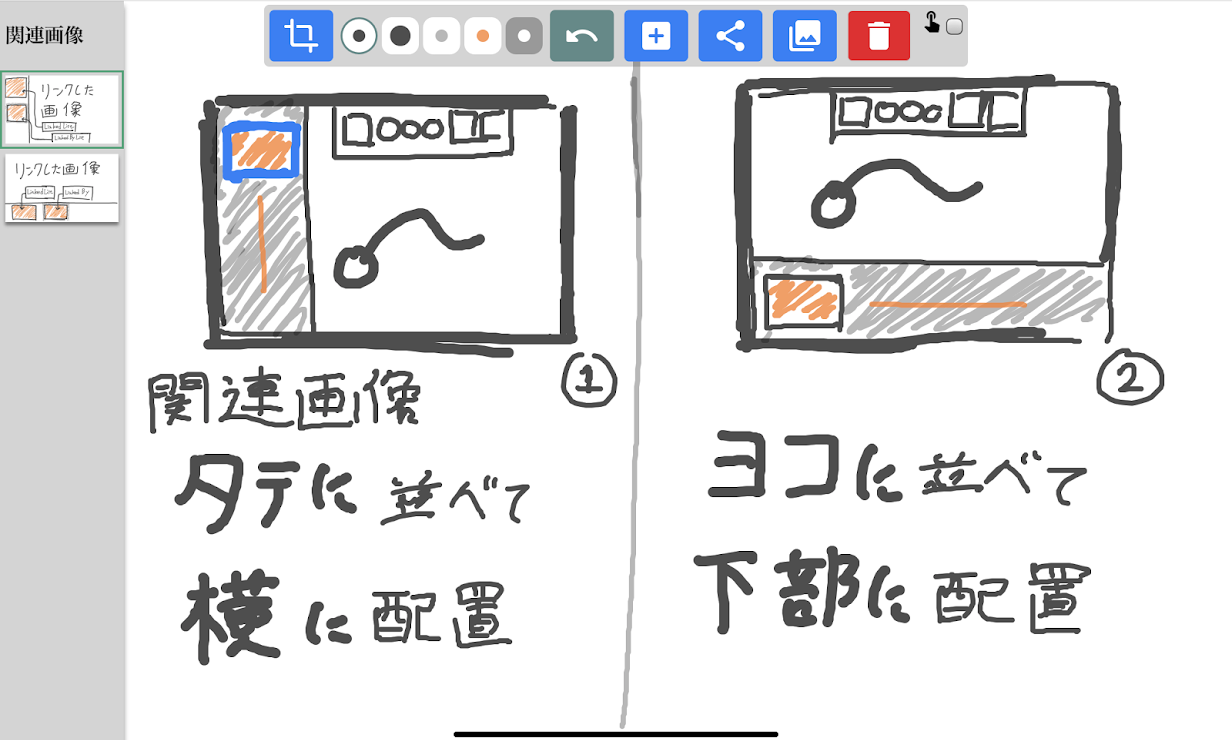
\includegraphics[width=70mm]{images/mockup1.png}}
                      \end{center} \caption{DrawWikを用いて作成されたDrawwikiのモックアップ} \label{fig:protodrawwiki1}
\end{minipage} \begin{minipage}{0.5\hsize}
                   \begin{center} \fbox {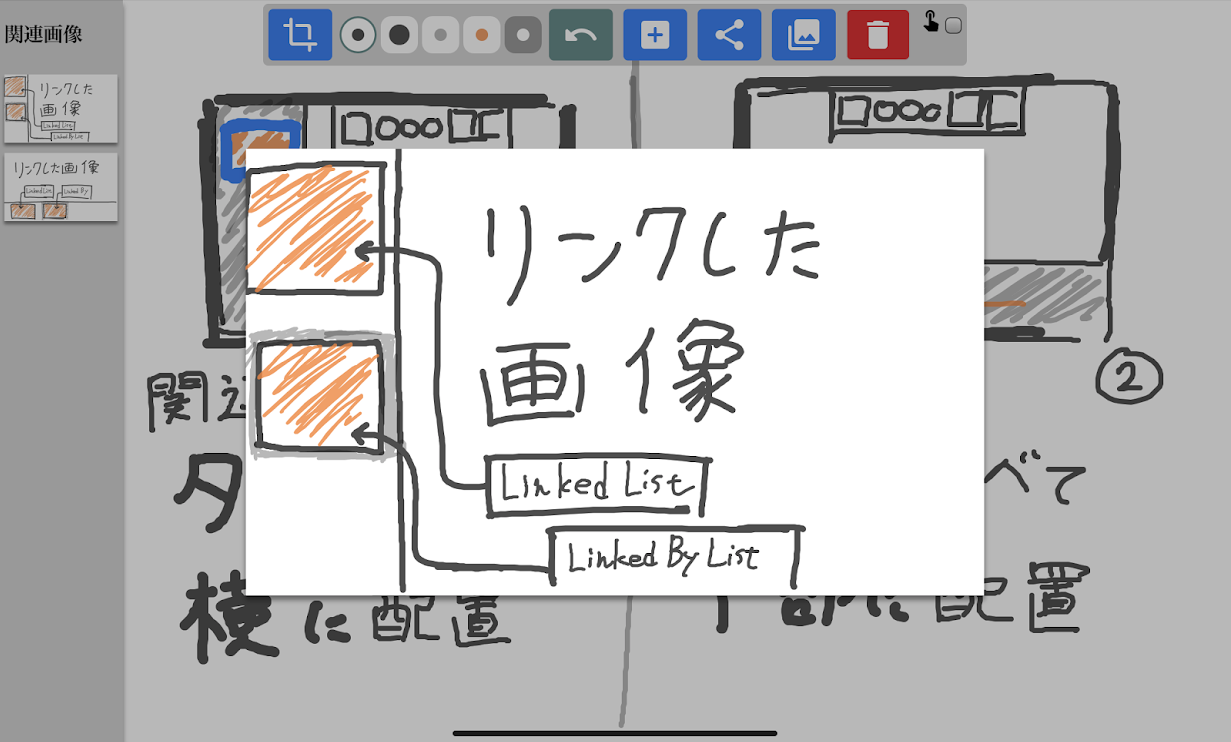
\includegraphics[width=70mm]{images/mockup2.png}}
                   \end{center} \caption{アクションによってポップアップするダイアログの再現} \label{fig:protodrawwiki2}
\end{minipage}
\end{figure}


\section{インタラクティブな図解}
\label{drawiki:zukai}
自動車等の整備を行う際は、製品マニュアルを熟読することで構造を理解し、交換すべき部品をパーツリストで確認し、さらに
取り付けに必要なワッシャ・ボルトのサイズやそれらの適正な締め付けトルクを念頭に置いた上で行う必要があるが、それらの情報は
異なるページや冊子に分かれて記載されていることが一般的であり、参照が大変である。(図\ref{fig:partslist}, 図\ref{fig:manual})

\begin{figure}[H] \begin{minipage}{0.5\hsize}
                      \begin{center} \fbox {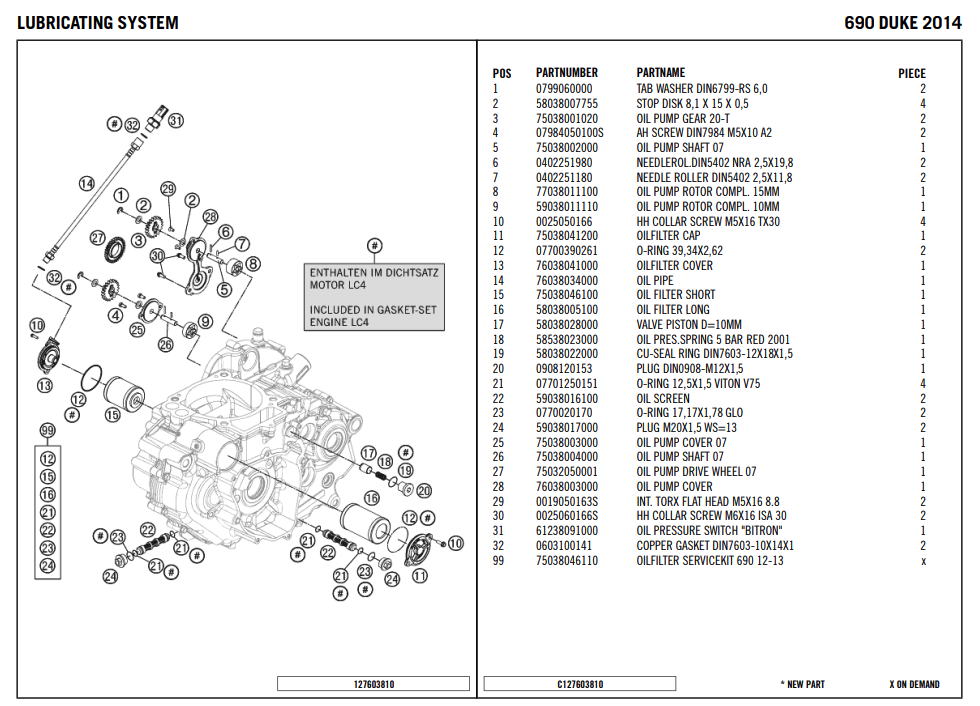
\includegraphics[width=70mm]{images/partslist.png}}
                      \end{center} \caption{既存のパーツリスト} \label{fig:partslist}
\end{minipage} \begin{minipage}{0.5\hsize}
                   \begin{center} \fbox {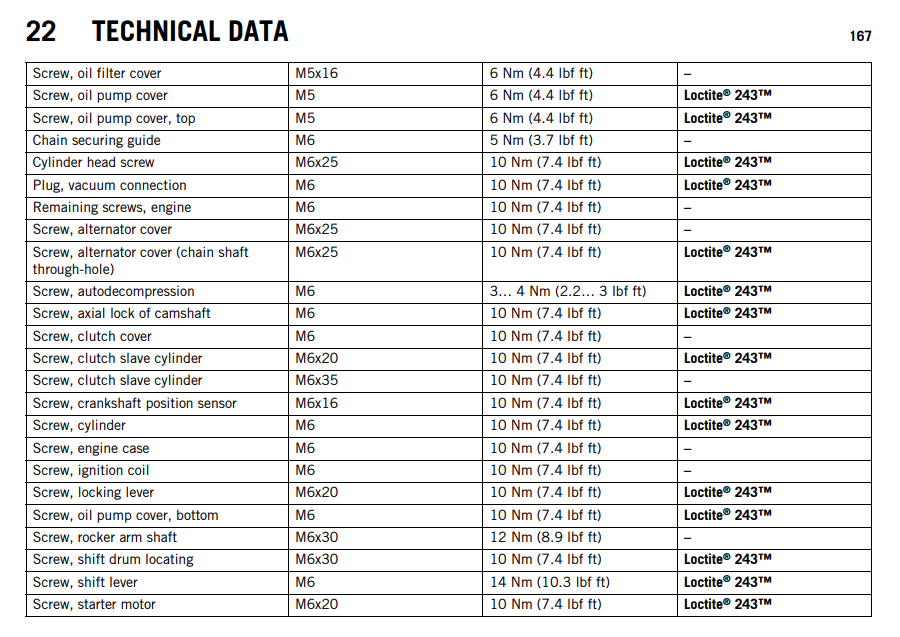
\includegraphics[width=70mm]{images/manual1.png}}
                   \end{center} \caption{既存の部品情報リスト} \label{fig:manual}
\end{minipage}
\end{figure}

\begin{figure}[H] \begin{minipage}{0.5\hsize}
                      \begin{center} \fbox {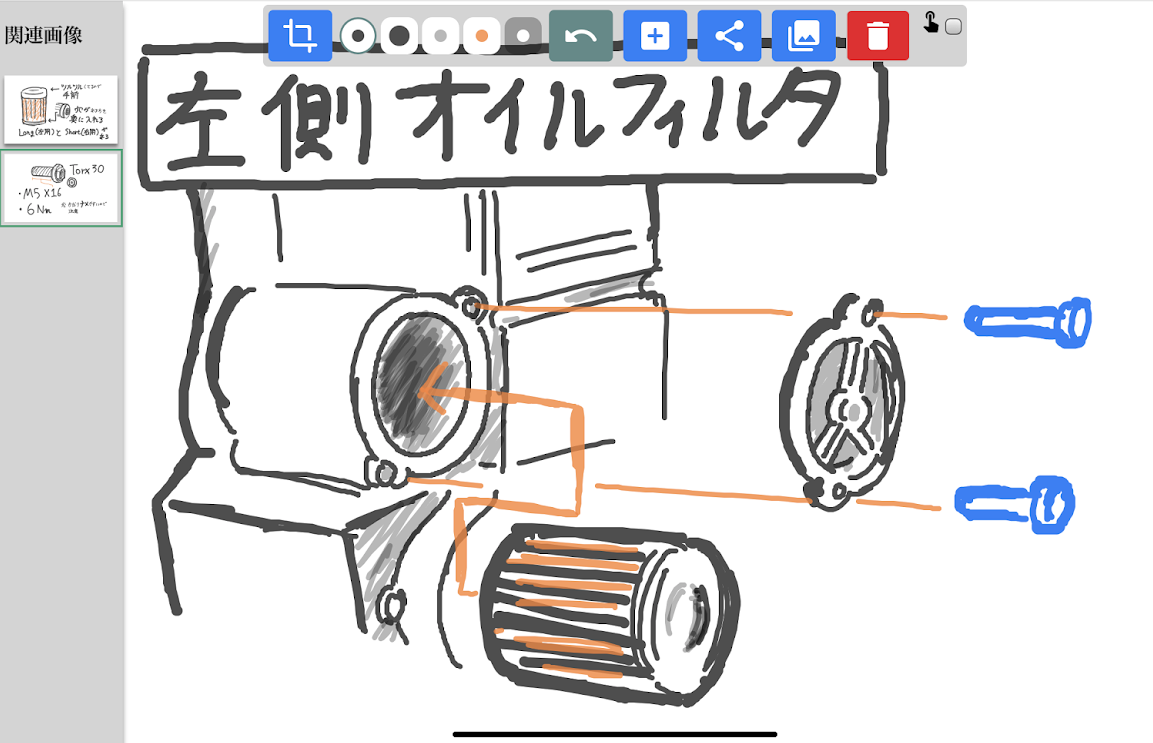
\includegraphics[width=70mm]{images/mymanual1.png}}
                      \end{center} \caption{DrawWikiによる自作整備メモ} \label{fig:oremanual1}
\end{minipage} \begin{minipage}{0.5\hsize}
                   \begin{center} \fbox {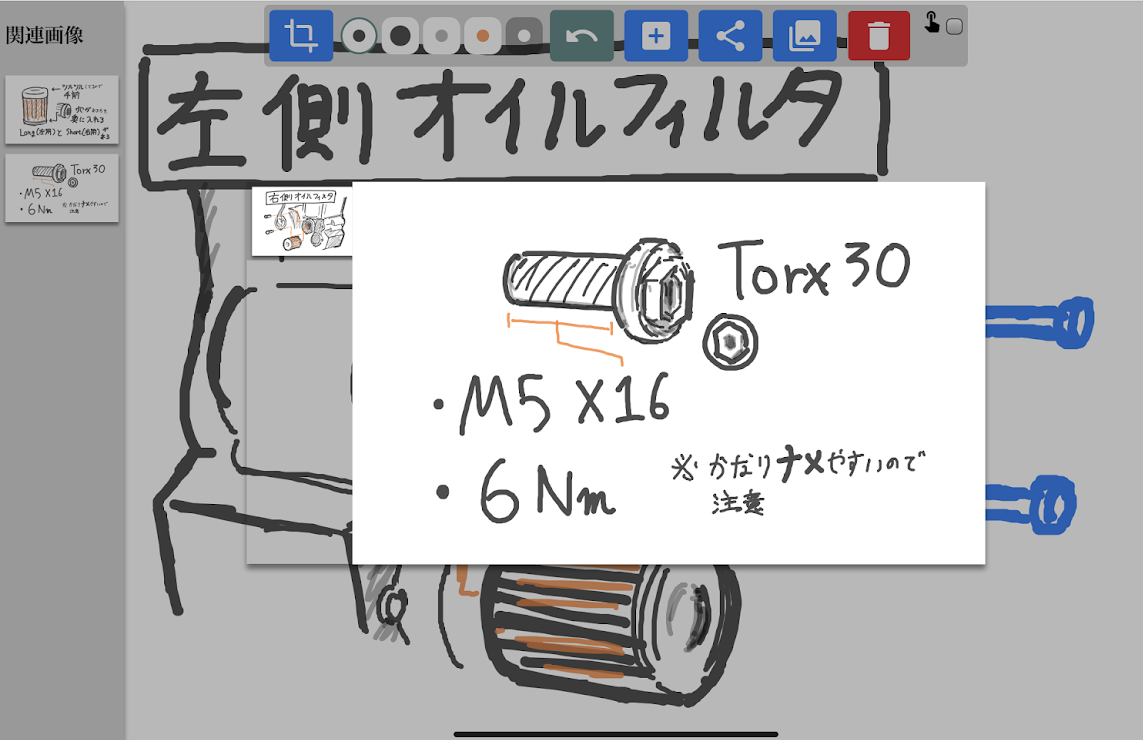
\includegraphics[width=70mm]{images/mymanual2.png}}
                   \end{center} \caption{関連情報を表示した画面} \label{fig:oremanual2}
\end{minipage}
\end{figure}

DrawWikiでは製品の構造を理解しやすいよう自由なレイアウトで簡潔に書いた図に 部品や組み立てに要する注意等のリストが描かれた別のメモをリンクさせることで、
必要な情報へ素早くアクセスする手段を確保しながら、画面が注釈で埋まることのない視認性に優れた図解を作成することが可能である。
またリンク構造によって同じ部品や工具を用いる他のメモも推薦されるため、整備の手順を考える手助けとなる効果もある。

\section{リンクに基づいたフラットな手書きメモの管理}
これらのメモは全く異なる分野を取り扱ったものであり、従来のメモアプリケーションでは異なるフォルダに格納する、
またはタグやラベル等を貼り付ける等の手段で分類されるべきものだったが、ハイパーイラスト内のリンク情報に基づいて関連イラストが
表示されるDrawWikiでは、情報の整理や適切な管理を特別心かげなくてもリンクを辿ることで目的のハイパーイラストを参照することが可能である。

\section{ナレッジの共有と共同編集}
DrawWikiによって作成されたハイパーイラストにはURLが割り振られているため、画像として他のWebサイト内に埋めこむことも可能である。
この状態でもリンク情報は失われずファイル内に内包されているため、リンクされている関連画像も含めたナレッジとして共有することができる。
さらに他のユーザーによる内容の追記や、別のハイパーイラストをリンクさせるといった操作にも対応しているため
手書きメモを取るような気軽さでWikiのようなコラボレーションを行うことができる。

%
%\section{手書きによるWebページ・Wikiの作成}
%\label{tegakiwiki}
%ハイパーイラストはそれ自体がハイパーリンクを内包したハイパーテキストであるため
%手書きという簡単な操作のみでWebページを作り、公開することができる。
%%\subsubsection{手書きベースWikiの優位性}
%通常のテキストベースのWikiはテキストによって内容を記述することを前提としているが、
%テキスト入力に起因する以下のような問題点がある。
%\begin{enumerate}
%    \item 効率的なテキスト入力はキーボード等の専用ハードウェアが必要であり、これらのデバイスを備えていないスマートフォンやタブレット等のハードウェアで便利に入力することができない
%    \item キーボードの操作にはタッチタイピング等の技術に習熟している必要があるため、利用者にはある程度の技能が要求されてしまう。
%    \item Wikiコンテンツの記述には専用の記法に倣う必要がある。例えばハイパーテキストを記述する上で代表的な言語であるHTMLでは、テキストへのハイパーリンクの埋め込みを以下のように定義する。
%    \begin{lstlisting}[caption=htmlにおけるハイパーリンクの定義, label=htmlhyperlinking]
%        <a href="https://example.com">HyperLink</a>
%    \end{lstlisting}
%    またHTMLへと変換できるプレーンテキストのフォーマットとして広く普及しているMarkdownでは、同様の構造を以下のように記述する。
%    \begin{lstlisting}[caption=MarkDownにおけるハイパーリンクの定義, label=mdhyperlinking]
%        [HyperLink]("https://example.com")
%    \end{lstlisting}
%    上記の記法とは別に独自の記法を採用しているWikiも存在するため、その各々の記法も利用者は網羅していなければならない。
%\end{enumerate}
%
%(1)についてはタッチパネルさえあれば手書き入力が可能であるため、スマートフォンやタブレット等のキーボードを持たないデバイスからでも利用することができる。
%(2)に関しても、手書きはタイピングが登場する以前から存在する馴染み深いベーシックな入力方法であり、タッチタイピング等の技能を持たないが手書きはできる人でも利用することができる。
%ハイパーリンクの定義も作成も手書きとシンプルな操作で完結するため(3)のような記法を覚える必要もない。

\section{まとめ}
本章では、本システムによって実現可能な利用例について述べた。
ハイパーイラストと手書きベースWikiの組み合わせによって 既存の手書きメモ・イラストの問題点を解決でき、
またテキストベースWikiに対しても優れた点があることがわかった。
本章で述べた応用例に限らず、様々な応用が可能と考えられる。